% Options for packages loaded elsewhere
\PassOptionsToPackage{unicode}{hyperref}
\PassOptionsToPackage{hyphens}{url}
\PassOptionsToPackage{dvipsnames,svgnames,x11names}{xcolor}
%
\documentclass[
  dvipsnames]{article}
\title{SEIS 631 Final Project: Florence Nightingale \& Data Viz}
\author{Ellie Byler}
\date{5/15/2022}

\usepackage{amsmath,amssymb}
\usepackage{lmodern}
\usepackage{iftex}
\ifPDFTeX
  \usepackage[T1]{fontenc}
  \usepackage[utf8]{inputenc}
  \usepackage{textcomp} % provide euro and other symbols
\else % if luatex or xetex
  \usepackage{unicode-math}
  \defaultfontfeatures{Scale=MatchLowercase}
  \defaultfontfeatures[\rmfamily]{Ligatures=TeX,Scale=1}
\fi
% Use upquote if available, for straight quotes in verbatim environments
\IfFileExists{upquote.sty}{\usepackage{upquote}}{}
\IfFileExists{microtype.sty}{% use microtype if available
  \usepackage[]{microtype}
  \UseMicrotypeSet[protrusion]{basicmath} % disable protrusion for tt fonts
}{}
\makeatletter
\@ifundefined{KOMAClassName}{% if non-KOMA class
  \IfFileExists{parskip.sty}{%
    \usepackage{parskip}
  }{% else
    \setlength{\parindent}{0pt}
    \setlength{\parskip}{6pt plus 2pt minus 1pt}}
}{% if KOMA class
  \KOMAoptions{parskip=half}}
\makeatother
\usepackage{xcolor}
\IfFileExists{xurl.sty}{\usepackage{xurl}}{} % add URL line breaks if available
\IfFileExists{bookmark.sty}{\usepackage{bookmark}}{\usepackage{hyperref}}
\hypersetup{
  pdftitle={SEIS 631 Final Project: Florence Nightingale \& Data Viz},
  pdfauthor={Ellie Byler},
  colorlinks=true,
  linkcolor={Maroon},
  filecolor={Maroon},
  citecolor={Blue},
  urlcolor={blue},
  pdfcreator={LaTeX via pandoc}}
\urlstyle{same} % disable monospaced font for URLs
\usepackage[margin=1in]{geometry}
\usepackage{color}
\usepackage{fancyvrb}
\newcommand{\VerbBar}{|}
\newcommand{\VERB}{\Verb[commandchars=\\\{\}]}
\DefineVerbatimEnvironment{Highlighting}{Verbatim}{commandchars=\\\{\}}
% Add ',fontsize=\small' for more characters per line
\usepackage{framed}
\definecolor{shadecolor}{RGB}{248,248,248}
\newenvironment{Shaded}{\begin{snugshade}}{\end{snugshade}}
\newcommand{\AlertTok}[1]{\textcolor[rgb]{0.94,0.16,0.16}{#1}}
\newcommand{\AnnotationTok}[1]{\textcolor[rgb]{0.56,0.35,0.01}{\textbf{\textit{#1}}}}
\newcommand{\AttributeTok}[1]{\textcolor[rgb]{0.77,0.63,0.00}{#1}}
\newcommand{\BaseNTok}[1]{\textcolor[rgb]{0.00,0.00,0.81}{#1}}
\newcommand{\BuiltInTok}[1]{#1}
\newcommand{\CharTok}[1]{\textcolor[rgb]{0.31,0.60,0.02}{#1}}
\newcommand{\CommentTok}[1]{\textcolor[rgb]{0.56,0.35,0.01}{\textit{#1}}}
\newcommand{\CommentVarTok}[1]{\textcolor[rgb]{0.56,0.35,0.01}{\textbf{\textit{#1}}}}
\newcommand{\ConstantTok}[1]{\textcolor[rgb]{0.00,0.00,0.00}{#1}}
\newcommand{\ControlFlowTok}[1]{\textcolor[rgb]{0.13,0.29,0.53}{\textbf{#1}}}
\newcommand{\DataTypeTok}[1]{\textcolor[rgb]{0.13,0.29,0.53}{#1}}
\newcommand{\DecValTok}[1]{\textcolor[rgb]{0.00,0.00,0.81}{#1}}
\newcommand{\DocumentationTok}[1]{\textcolor[rgb]{0.56,0.35,0.01}{\textbf{\textit{#1}}}}
\newcommand{\ErrorTok}[1]{\textcolor[rgb]{0.64,0.00,0.00}{\textbf{#1}}}
\newcommand{\ExtensionTok}[1]{#1}
\newcommand{\FloatTok}[1]{\textcolor[rgb]{0.00,0.00,0.81}{#1}}
\newcommand{\FunctionTok}[1]{\textcolor[rgb]{0.00,0.00,0.00}{#1}}
\newcommand{\ImportTok}[1]{#1}
\newcommand{\InformationTok}[1]{\textcolor[rgb]{0.56,0.35,0.01}{\textbf{\textit{#1}}}}
\newcommand{\KeywordTok}[1]{\textcolor[rgb]{0.13,0.29,0.53}{\textbf{#1}}}
\newcommand{\NormalTok}[1]{#1}
\newcommand{\OperatorTok}[1]{\textcolor[rgb]{0.81,0.36,0.00}{\textbf{#1}}}
\newcommand{\OtherTok}[1]{\textcolor[rgb]{0.56,0.35,0.01}{#1}}
\newcommand{\PreprocessorTok}[1]{\textcolor[rgb]{0.56,0.35,0.01}{\textit{#1}}}
\newcommand{\RegionMarkerTok}[1]{#1}
\newcommand{\SpecialCharTok}[1]{\textcolor[rgb]{0.00,0.00,0.00}{#1}}
\newcommand{\SpecialStringTok}[1]{\textcolor[rgb]{0.31,0.60,0.02}{#1}}
\newcommand{\StringTok}[1]{\textcolor[rgb]{0.31,0.60,0.02}{#1}}
\newcommand{\VariableTok}[1]{\textcolor[rgb]{0.00,0.00,0.00}{#1}}
\newcommand{\VerbatimStringTok}[1]{\textcolor[rgb]{0.31,0.60,0.02}{#1}}
\newcommand{\WarningTok}[1]{\textcolor[rgb]{0.56,0.35,0.01}{\textbf{\textit{#1}}}}
\usepackage{graphicx}
\makeatletter
\def\maxwidth{\ifdim\Gin@nat@width>\linewidth\linewidth\else\Gin@nat@width\fi}
\def\maxheight{\ifdim\Gin@nat@height>\textheight\textheight\else\Gin@nat@height\fi}
\makeatother
% Scale images if necessary, so that they will not overflow the page
% margins by default, and it is still possible to overwrite the defaults
% using explicit options in \includegraphics[width, height, ...]{}
\setkeys{Gin}{width=\maxwidth,height=\maxheight,keepaspectratio}
% Set default figure placement to htbp
\makeatletter
\def\fps@figure{htbp}
\makeatother
\setlength{\emergencystretch}{3em} % prevent overfull lines
\providecommand{\tightlist}{%
  \setlength{\itemsep}{0pt}\setlength{\parskip}{0pt}}
\setcounter{secnumdepth}{-\maxdimen} % remove section numbering
\ifLuaTeX
  \usepackage{selnolig}  % disable illegal ligatures
\fi

\begin{document}
\maketitle

\hypertarget{section}{%
\section{\texorpdfstring{\textcolor{WildStrawberry}{INTRODUCTION}}{}}\label{section}}

\textbf{\href{https://en.wikipedia.org/wiki/Florence_Nightingale}{Florence
Nightingale}} (1820-1910) was an incredible woman. Not only did she
revolutionize medical care by setting the standards for modern nursing,
she also was a pioneer in the field of statistics and especially data
visualization. Working at a military hospital during the
\href{https://en.wikipedia.org/wiki/Crimean_War}{Crimean War},
Nightingale was struck by the deplorable conditions for wounded
soldiers. She suspected that many of them were dying from diseases that
would be preventable with proper hygiene protocols. Determined to
convince the British government that something had to change,
Nightingale collected data and drew up charts to accompany her
\href{https://curiosity.lib.harvard.edu/contagion/catalog/36-990101646750203941}{report}.
Data visualization was still novel at the time, and Nightingale's charts
allowed her to proscribe a solution instead of merely describing the
problem. She became the first female member elected to the Royal
Statistical Society in 1859.

\hypertarget{section-1}{%
\subsection{\texorpdfstring{\textcolor{TealBlue}{What:}}{}}\label{section-1}}

My goal for this project was to create an R Shiny dashboard celebrating
Florence Nightingale's contributions to stats and data analysis and
exploring her work.

\hypertarget{section-2}{%
\subsection{\texorpdfstring{\textcolor{TealBlue}{Why:}}{}}\label{section-2}}

Florence Nightingale is arguably the mother of data viz, and I thought
it would be interesting to see what sort of modern data visualizations I
could create using her
\href{https://github.com/vincentarelbundock/Rdatasets/blob/master/csv/HistData/Nightingale.csv}{historical
data}. I also wanted more people to know about this amazing woman who
deserves a place next to Ada Lovelace in the pantheon of influential
women in STEM.

\hypertarget{section-3}{%
\subsection{\texorpdfstring{\textcolor{TealBlue}{How:}}{}}\label{section-3}}

Using Florence Nightingale's data that she collected during her time at
the military hospital, I created a web app using R Shiny that allows
users to see her original data visualizations next to modern
recreations.

\newpage

\hypertarget{section-4}{%
\section{\texorpdfstring{\textcolor{WildStrawberry}{CREATING THE APP}}{}}\label{section-4}}

\textbf{Link to the app:
\url{https://e11i3n0r.shinyapps.io/631-EllieByler-FinalProject/}}

\begin{center}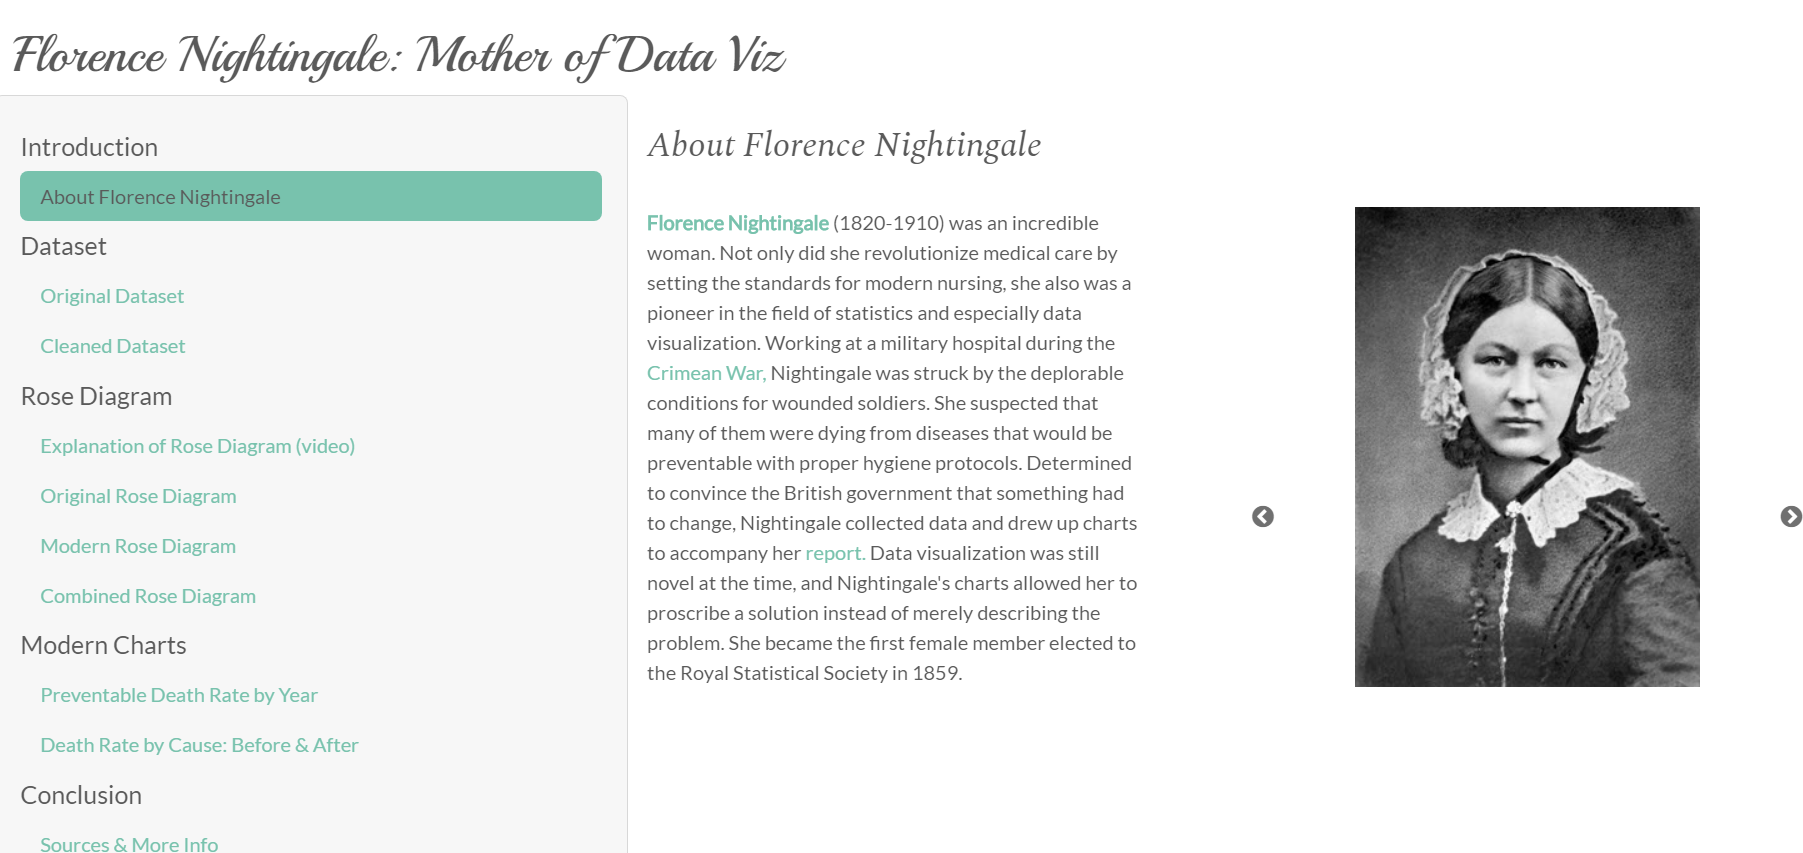
\includegraphics[width=1\linewidth]{app_landing_page} \end{center}

\hypertarget{section-5}{%
\subsection{\texorpdfstring{\textcolor{TealBlue}{Getting Started:}}{}}\label{section-5}}

Creating an app using R Shiny is surprisingly simple. First, install the
Shiny package using \texttt{install.packages("shiny")} in your R
console. Select \texttt{File\ →\ New\ File\ →\ Shiny\ Web\ App} in
RStudio and save it to a new folder directory on your computer.

\begin{center}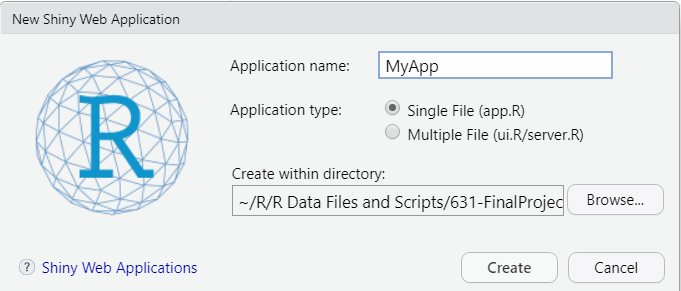
\includegraphics[width=0.6\linewidth]{app_create_new} \end{center}

Here is the minimal code necessary to create a functioning app:

\begin{Shaded}
\begin{Highlighting}[]
\CommentTok{\# use install.packages(\textquotesingle{}shiny\textquotesingle{}) first if it\textquotesingle{}s not}
\CommentTok{\# installed}

\FunctionTok{library}\NormalTok{(shiny)}

\CommentTok{\# UI SECTION}
\NormalTok{ui }\OtherTok{\textless{}{-}} \FunctionTok{fluidPage}\NormalTok{(}\StringTok{"Hello, world!"}\NormalTok{)}

\CommentTok{\# SERVER SECTION}
\NormalTok{server }\OtherTok{\textless{}{-}} \ControlFlowTok{function}\NormalTok{(input, output) \{}
\NormalTok{\}}

\FunctionTok{shinyApp}\NormalTok{(ui, server)}
\end{Highlighting}
\end{Shaded}

There are only two main components: the UI and the Server. Of course,
within that basic framework, there is much room for added customization
and complexity. I was able to format a navigation sidebar, include data
tables and graphs, embed videos and audio, and use a custom theme
(\href{https://bootswatch.com/minty/}{Bootswatch: ``Minty''}) and fonts.

\hypertarget{section-6}{%
\subsection{\texorpdfstring{\textcolor{TealBlue}{Cleaning and Prepping the Data:}}{}}\label{section-6}}

I found a dataset on Github of Florence Nightingale's data collected
over two years during her time as a nurse in the Crimean War. It is a
small dataset with only 24 records (each record represents a month),
which goes to show that even limited datasets can prove useful for
analysis. Nightingale's original data table is shown below.

\textbf{Link to dataset:
\url{https://github.com/vincentarelbundock/Rdatasets/blob/master/csv/HistData/Nightingale.csv}}

\begin{center}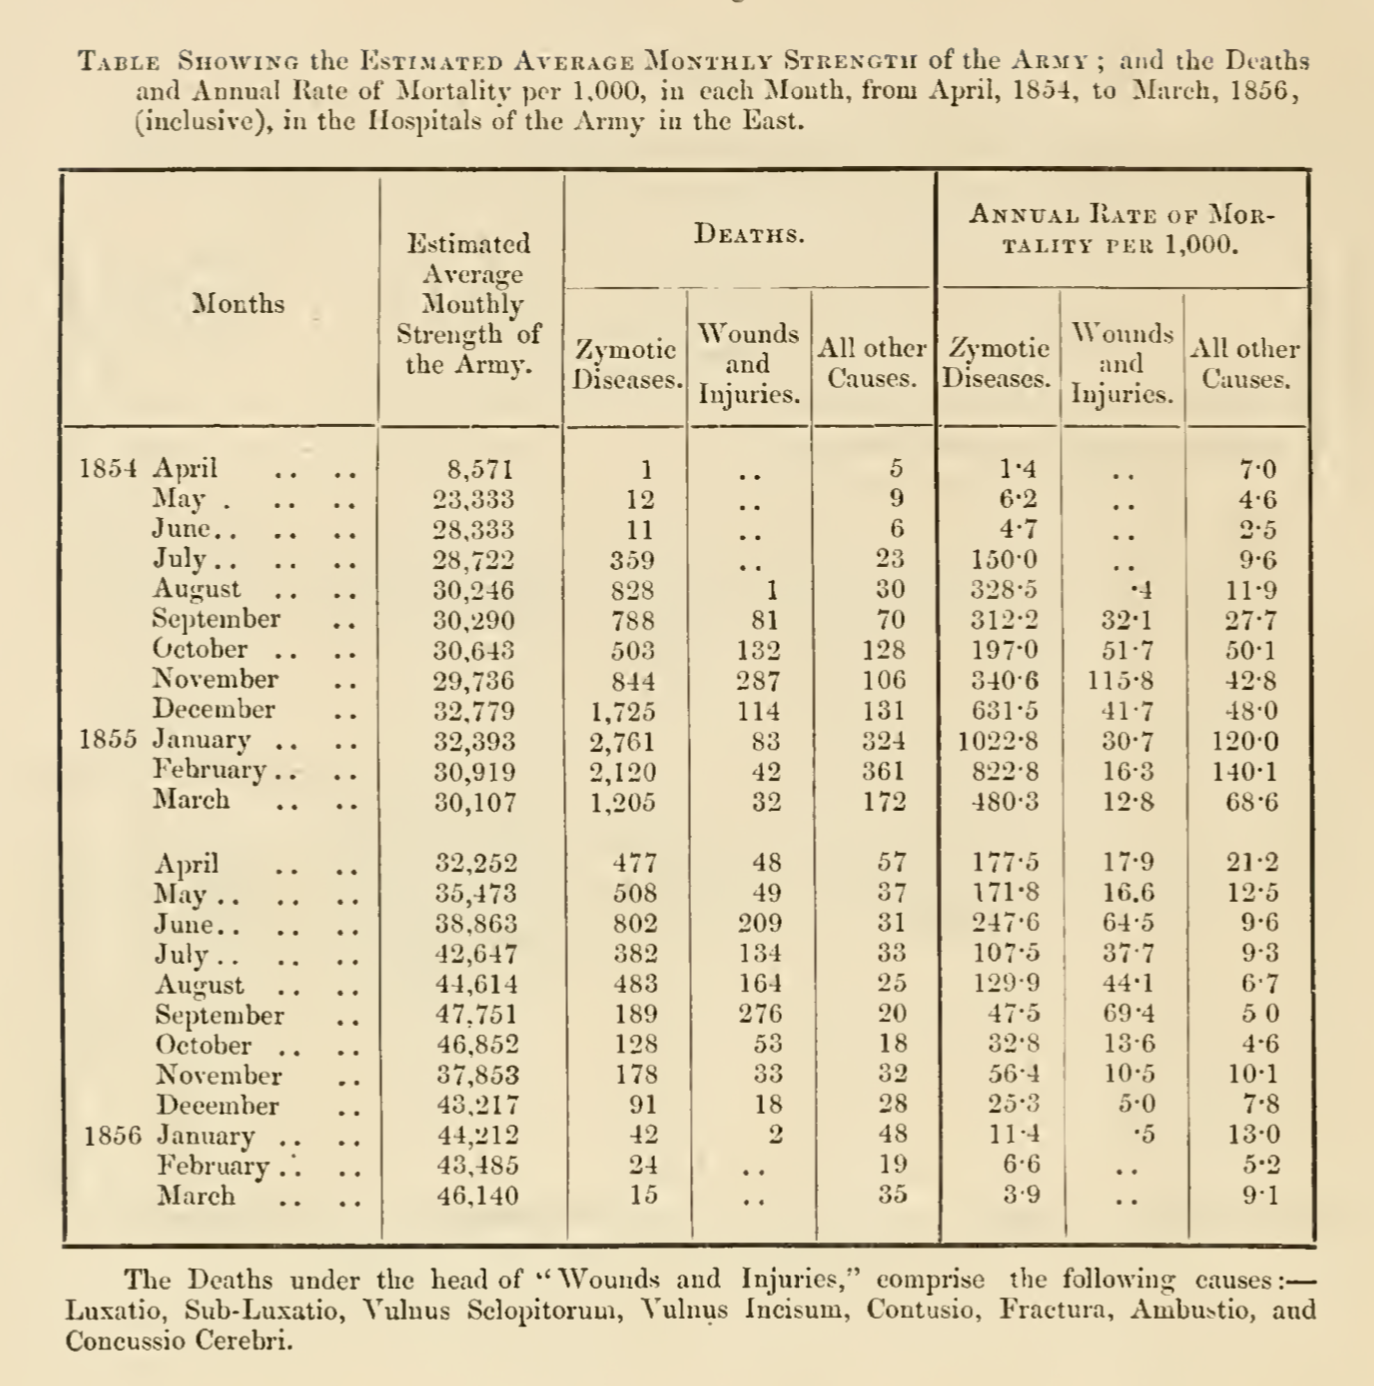
\includegraphics[width=0.8\linewidth]{florence_data_table} \end{center}

\newpage

\begin{Shaded}
\begin{Highlighting}[]
\CommentTok{\# LOAD DATA}

\FunctionTok{library}\NormalTok{(readxl)  }\CommentTok{\# for loading dataset from Excel file.}

\NormalTok{Nightingale }\OtherTok{\textless{}{-}} \FunctionTok{read\_excel}\NormalTok{(}\StringTok{"DATASET\_Nightingale.xlsx"}\NormalTok{,}
    \AttributeTok{sheet =} \StringTok{"Nightingale"}\NormalTok{)}
\end{Highlighting}
\end{Shaded}

After loading the dataset, it needed substantial modifications to make
the types of charts that I needed.

\begin{Shaded}
\begin{Highlighting}[]
\CommentTok{\# PREP DATA FOR ANALYSIS}

\FunctionTok{library}\NormalTok{(magrittr)  }\CommentTok{\# adds operators that make function sequencing easier.}
\FunctionTok{library}\NormalTok{(tidyverse)  }\CommentTok{\# for data manipulation and visualization.}
\FunctionTok{library}\NormalTok{(stringr)  }\CommentTok{\# for text processing.}
\FunctionTok{library}\NormalTok{(zoo)  }\CommentTok{\# for date{-}time processing.}
\FunctionTok{library}\NormalTok{(lubridate)  }\CommentTok{\# for date{-}time processing.}

\NormalTok{Nightingale }\SpecialCharTok{\%\textgreater{}\%}
    \FunctionTok{select}\NormalTok{(}\SpecialCharTok{{-}}\FunctionTok{c}\NormalTok{(}\StringTok{"ID"}\NormalTok{)) }\SpecialCharTok{\%\textgreater{}\%}
    \FunctionTok{pivot\_longer}\NormalTok{(}\AttributeTok{cols =} \FunctionTok{c}\NormalTok{(}\StringTok{"Disease"}\NormalTok{, }\StringTok{"Wounds"}\NormalTok{, }\StringTok{"Other"}\NormalTok{),}
        \AttributeTok{names\_to =} \FunctionTok{c}\NormalTok{(}\StringTok{"Cause"}\NormalTok{), }\AttributeTok{values\_to =} \FunctionTok{c}\NormalTok{(}\StringTok{"Deaths"}\NormalTok{)) }\SpecialCharTok{\%\textgreater{}\%}
    \FunctionTok{mutate}\NormalTok{(}\AttributeTok{Rate =} \FunctionTok{if\_else}\NormalTok{(.}\SpecialCharTok{$}\NormalTok{Cause }\SpecialCharTok{==} \StringTok{"Disease"}\NormalTok{, .}\SpecialCharTok{$}\NormalTok{Disease.rate,}
        \FunctionTok{if\_else}\NormalTok{(.}\SpecialCharTok{$}\NormalTok{Cause }\SpecialCharTok{==} \StringTok{"Wounds"}\NormalTok{, .}\SpecialCharTok{$}\NormalTok{Wounds.rate,}
\NormalTok{            .}\SpecialCharTok{$}\NormalTok{Other.rate))) }\SpecialCharTok{\%\textgreater{}\%}
    \FunctionTok{select}\NormalTok{(}\SpecialCharTok{{-}}\FunctionTok{c}\NormalTok{(}\StringTok{"Disease.rate"}\NormalTok{, }\StringTok{"Wounds.rate"}\NormalTok{, }\StringTok{"Other.rate"}\NormalTok{)) }\SpecialCharTok{\%\textgreater{}\%}
    \FunctionTok{mutate}\NormalTok{(}\AttributeTok{Rate =} \FunctionTok{round}\NormalTok{((Rate}\SpecialCharTok{/}\DecValTok{12}\NormalTok{), }\DecValTok{2}\NormalTok{)) }\SpecialCharTok{\%\textgreater{}\%}
    \FunctionTok{unite}\NormalTok{(}\StringTok{"Month\_Year"}\NormalTok{, Month}\SpecialCharTok{:}\NormalTok{Year, }\AttributeTok{sep =} \StringTok{" "}\NormalTok{, }\AttributeTok{remove =} \ConstantTok{FALSE}\NormalTok{) }\SpecialCharTok{\%\textgreater{}\%}
    \FunctionTok{mutate}\NormalTok{(}\AttributeTok{Regime =} \FunctionTok{if\_else}\NormalTok{(}\FunctionTok{str\_detect}\NormalTok{(.}\SpecialCharTok{$}\NormalTok{Month\_Year,}
        \StringTok{"[:alpha:]}\SpecialCharTok{\textbackslash{}\textbackslash{}}\StringTok{s1854"}\NormalTok{), }\StringTok{"Before"}\NormalTok{, }\FunctionTok{if\_else}\NormalTok{(}\FunctionTok{str\_detect}\NormalTok{(.}\SpecialCharTok{$}\NormalTok{Month\_Year,}
        \StringTok{"(Jan|Feb|Mar)}\SpecialCharTok{\textbackslash{}\textbackslash{}}\StringTok{s1855"}\NormalTok{), }\StringTok{"Before"}\NormalTok{, }\StringTok{"After"}\NormalTok{))) }\SpecialCharTok{\%\textgreater{}\%}
    \FunctionTok{mutate}\NormalTok{(}\AttributeTok{Regime =} \FunctionTok{factor}\NormalTok{(Regime, }\AttributeTok{levels =} \FunctionTok{c}\NormalTok{(}\StringTok{"Before"}\NormalTok{,}
        \StringTok{"After"}\NormalTok{))) }\SpecialCharTok{\%\textgreater{}\%}
    \FunctionTok{mutate}\NormalTok{(}\AttributeTok{Sort\_Date =} \FunctionTok{as.yearmon}\NormalTok{(}\FunctionTok{as.Date}\NormalTok{(Date))) }\SpecialCharTok{\%\textgreater{}\%}
    \FunctionTok{mutate}\NormalTok{(}\AttributeTok{mo =} \FunctionTok{month}\NormalTok{(Date, }\AttributeTok{label =} \ConstantTok{TRUE}\NormalTok{, }\AttributeTok{abbr =} \ConstantTok{TRUE}\NormalTok{)) }\OtherTok{{-}\textgreater{}}
\NormalTok{    long\_data}
\end{Highlighting}
\end{Shaded}

The main things accomplished by the code above are pivoting the data so
that \texttt{Deaths}, \texttt{Cause}, and \texttt{Rate} are single
columns instead of having \texttt{Disease.rate}, \texttt{Wounds.rate},
etc. I also added a column called \texttt{Regime} that has values of
``\emph{Before}'' or ``\emph{After}'' based on the date. This refers to
when a Sanitary Commission arrived at the hospital in March 1855 to help
implement hygiene practices that drastically reduced preventable deaths
from disease among wounded soldiers.

\hypertarget{section-7}{%
\subsection{\texorpdfstring{\textcolor{TealBlue}{Data Visualizations:}}{}}\label{section-7}}

For reference, I've included the graphic that inspired this project on
the next page: Nightingale's famous chart depicting the causes of
mortality in the British army during the Crimean War from April 1854 to
March 1856. This \emph{rose diagram} is alternatively called a
\emph{coxcomb} or a \emph{polar area chart}.

\newpage

\hypertarget{florence-nightingales-original-rose-diagram-explanatory-text}{%
\subsubsection{\texorpdfstring{\emph{Florence Nightingale's Original
Rose Diagram \& Explanatory
Text:}}{Florence Nightingale's Original Rose Diagram \& Explanatory Text:}}\label{florence-nightingales-original-rose-diagram-explanatory-text}}

DIAGRAM of the CAUSES of MORTALITY in the ARMY in the EAST

Figure 1: APRIL 1854 to MARCH 1855\\
Figure 2: APRIL 1855 to MARCH 1856

\begin{center}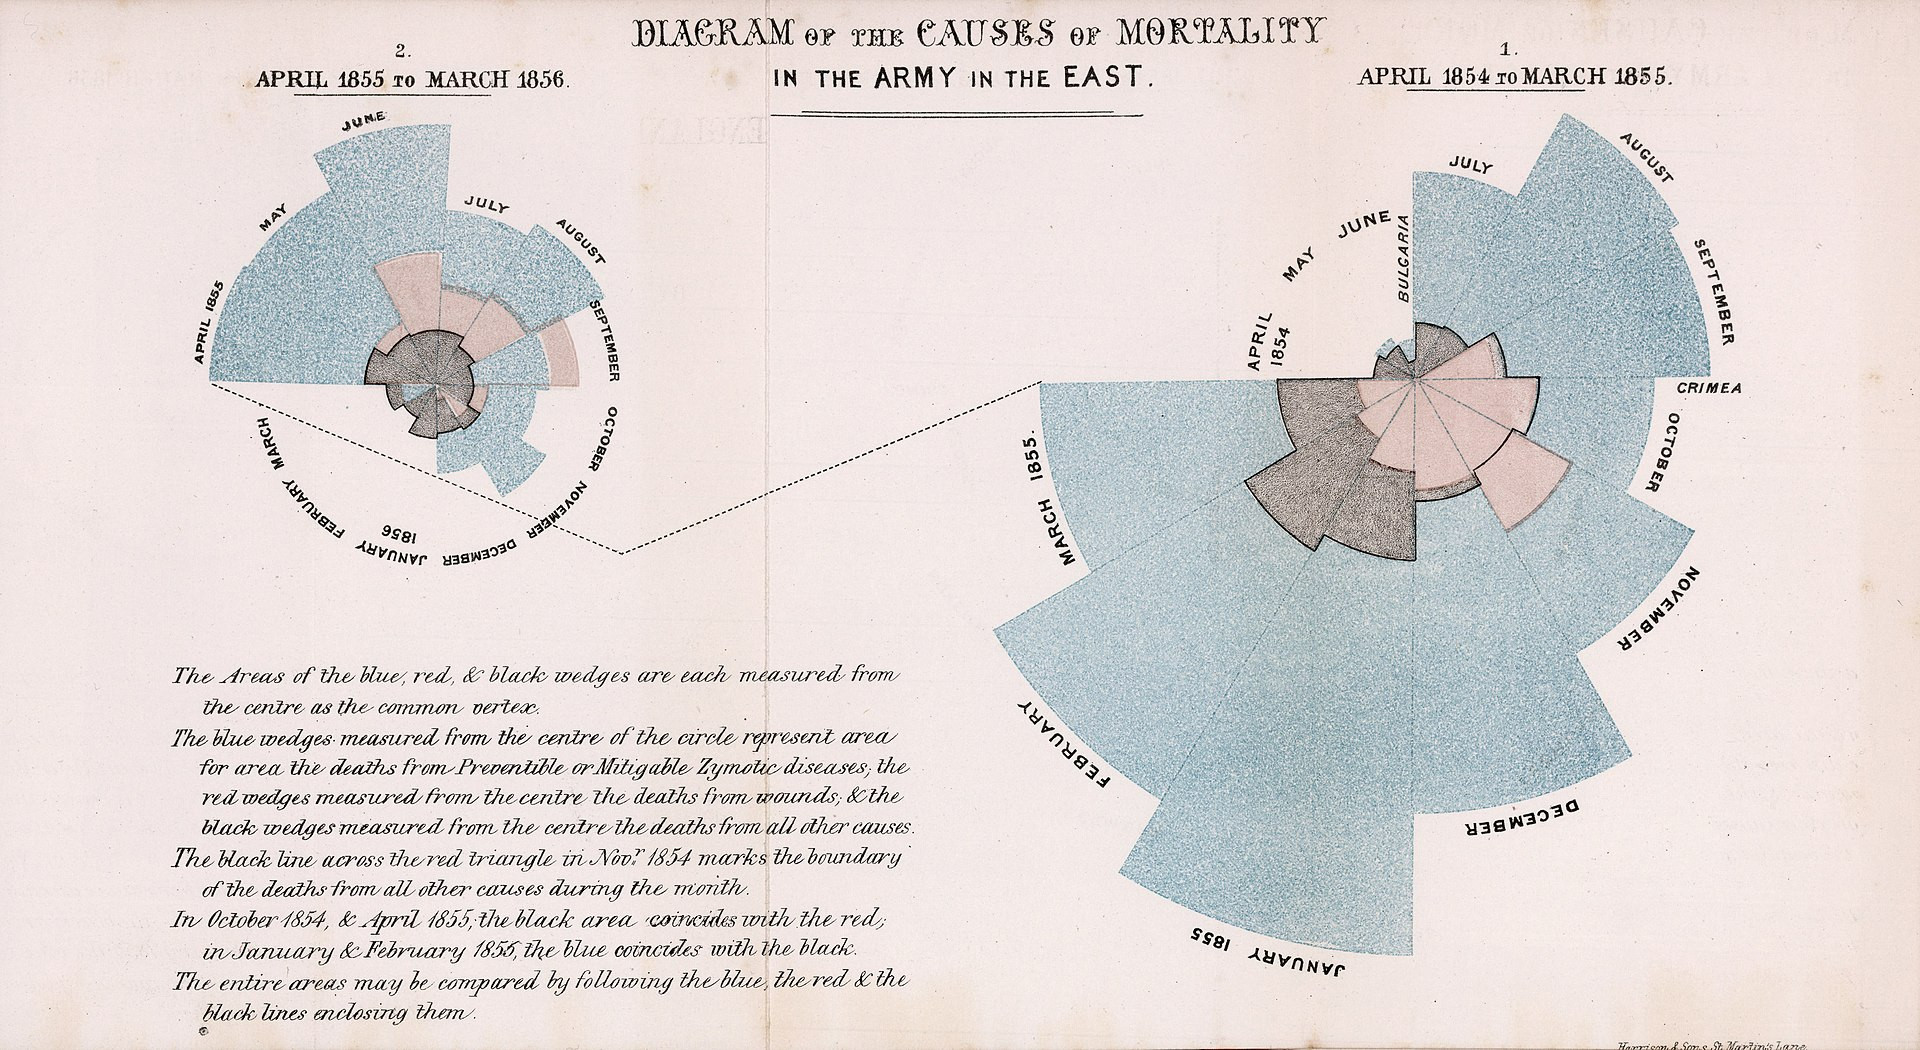
\includegraphics[width=0.9\linewidth]{Rose_Diagram_rmd} \end{center}

\begin{itemize}
\tightlist
\item
  The areas of the \textcolor{MidnightBlue}{blue},
  \textcolor{Sepia}{red}, \& black wedges are each measured from the
  center as the common vortex.
\item
  The \textcolor{MidnightBlue}{blue} wedges measured from the center of
  the circle represent area for area the deaths from
  \textcolor{MidnightBlue}{Preventable or Mitigable Zymotic diseases},
  the \textcolor{Sepia}{red} wedges measured from the center the deaths
  from \textcolor{Sepia}{wounds}, \& the black wedges measured from the
  center the deaths from all other causes.
\item
  The black line across the \textcolor{Sepia}{red} triangle in Nov.~1854
  marks the boundary of the deaths from all other causes during the
  month.
\item
  In October 1854 \& April 1855, the black area coincides with the the
  \textcolor{Sepia}{red}, in January \& February 1856, the
  \textcolor{MidnightBlue}{blue} coincides with the black.
\item
  The entire areas may be compared by following the
  \textcolor{MidnightBlue}{blue}, the \textcolor{Sepia}{red}, \& the
  black lines enclosing them.
\end{itemize}

\newpage

\hypertarget{modern-recreation-of-the-rose-diagram}{%
\subsubsection{\texorpdfstring{\emph{Modern Recreation of the Rose
Diagram}}{Modern Recreation of the Rose Diagram}}\label{modern-recreation-of-the-rose-diagram}}

For my first recreation of the rose diagram using R, I modified code
from this site: \url{https://rpubs.com/chidungkt/819554}. This is a
fairly faithful copy of the original, with similar coloring and layout.
The main differences are that the ``\emph{Before}'' panel has been moved
to the left of the ``\emph{After}'' panel, since this makes more sense
with how people tend to think about the passage of time. The graphs are
also flipped on the horizontal axis, with January at the top of the
circle instead of at the bottom. I discovered that a rose
diagram/coxcomb plot is just a bar chart with polar coordinates.

\begin{Shaded}
\begin{Highlighting}[]
\CommentTok{\# MODERN ROSE DIAGRAM}
\NormalTok{long\_data }\SpecialCharTok{\%\textgreater{}\%}
    \FunctionTok{ggplot}\NormalTok{(}\FunctionTok{aes}\NormalTok{(}\AttributeTok{x =}\NormalTok{ mo, }\AttributeTok{y =}\NormalTok{ Deaths, }\AttributeTok{fill =}\NormalTok{ Cause)) }\SpecialCharTok{+}
    \FunctionTok{geom\_col}\NormalTok{(}\AttributeTok{color =} \StringTok{"grey20"}\NormalTok{) }\SpecialCharTok{+} \FunctionTok{scale\_fill\_manual}\NormalTok{(}\AttributeTok{values =} \FunctionTok{c}\NormalTok{(}\StringTok{"\#6cc3d5"}\NormalTok{,}
    \StringTok{"\#7C8083"}\NormalTok{, }\StringTok{"\#f3969a"}\NormalTok{), }\AttributeTok{name =} \StringTok{""}\NormalTok{) }\SpecialCharTok{+} \FunctionTok{scale\_y\_sqrt}\NormalTok{() }\SpecialCharTok{+}
    \FunctionTok{facet\_wrap}\NormalTok{(}\SpecialCharTok{\textasciitilde{}}\NormalTok{Regime) }\SpecialCharTok{+} \FunctionTok{coord\_equal}\NormalTok{(}\AttributeTok{ratio =} \DecValTok{1}\NormalTok{) }\SpecialCharTok{+}
    \FunctionTok{coord\_polar}\NormalTok{() }\SpecialCharTok{+} \FunctionTok{labs}\NormalTok{(}\AttributeTok{title =} \StringTok{"Causes of Mortality in the Army in the East"}\NormalTok{,}
    \AttributeTok{subtitle =} \StringTok{"BEFORE and AFTER March 1855"}\NormalTok{, }\AttributeTok{caption =} \StringTok{"Data Source: Deaths from various causes in the Crimean War"}\NormalTok{) }\SpecialCharTok{+}
    \FunctionTok{theme}\NormalTok{(}\AttributeTok{legend.position =} \StringTok{"top"}\NormalTok{) }\SpecialCharTok{+} \FunctionTok{theme}\NormalTok{(}\AttributeTok{text =} \FunctionTok{element\_text}\NormalTok{(}\AttributeTok{size =} \DecValTok{12}\NormalTok{)) }\SpecialCharTok{+}
    \FunctionTok{theme}\NormalTok{(}\AttributeTok{axis.title.y =} \FunctionTok{element\_blank}\NormalTok{()) }\SpecialCharTok{+} \FunctionTok{theme}\NormalTok{(}\AttributeTok{axis.title.x =} \FunctionTok{element\_blank}\NormalTok{()) }\SpecialCharTok{+}
    \FunctionTok{theme}\NormalTok{(}\AttributeTok{axis.text.y =} \FunctionTok{element\_blank}\NormalTok{()) }\SpecialCharTok{+} \FunctionTok{theme}\NormalTok{(}\AttributeTok{axis.ticks =} \FunctionTok{element\_blank}\NormalTok{()) }\SpecialCharTok{+}
    \FunctionTok{theme}\NormalTok{(}\AttributeTok{plot.margin =} \FunctionTok{unit}\NormalTok{(}\FunctionTok{rep}\NormalTok{(}\FloatTok{0.7}\NormalTok{, }\DecValTok{4}\NormalTok{), }\StringTok{"cm"}\NormalTok{)) }\SpecialCharTok{+}
    \FunctionTok{theme}\NormalTok{(}\AttributeTok{plot.title =} \FunctionTok{element\_text}\NormalTok{(}\AttributeTok{color =} \StringTok{"\#78c2ad"}\NormalTok{,}
        \AttributeTok{size =} \DecValTok{16}\NormalTok{, }\AttributeTok{face =} \StringTok{"bold"}\NormalTok{)) }\SpecialCharTok{+} \FunctionTok{theme}\NormalTok{(}\AttributeTok{plot.caption =} \FunctionTok{element\_text}\NormalTok{(}\AttributeTok{color =} \StringTok{"grey70"}\NormalTok{,}
    \AttributeTok{size =} \DecValTok{10}\NormalTok{)) }\SpecialCharTok{+} \FunctionTok{theme}\NormalTok{(}\AttributeTok{plot.subtitle =} \FunctionTok{element\_text}\NormalTok{(}\AttributeTok{color =} \StringTok{"\#7C8083"}\NormalTok{,}
    \AttributeTok{size =} \DecValTok{12}\NormalTok{, }\AttributeTok{face =} \StringTok{"bold"}\NormalTok{)) }\SpecialCharTok{+} \FunctionTok{theme}\NormalTok{(}\AttributeTok{legend.text =} \FunctionTok{element\_text}\NormalTok{(}\AttributeTok{color =} \StringTok{"black"}\NormalTok{,}
    \AttributeTok{size =} \DecValTok{10}\NormalTok{)) }\SpecialCharTok{+} \FunctionTok{theme}\NormalTok{(}\AttributeTok{strip.text =} \FunctionTok{element\_text}\NormalTok{(}\AttributeTok{color =} \StringTok{"black"}\NormalTok{,}
    \AttributeTok{size =} \DecValTok{12}\NormalTok{, }\AttributeTok{face =} \StringTok{"bold"}\NormalTok{, }\AttributeTok{hjust =} \FloatTok{0.5}\NormalTok{))}
\end{Highlighting}
\end{Shaded}

\begin{flushleft}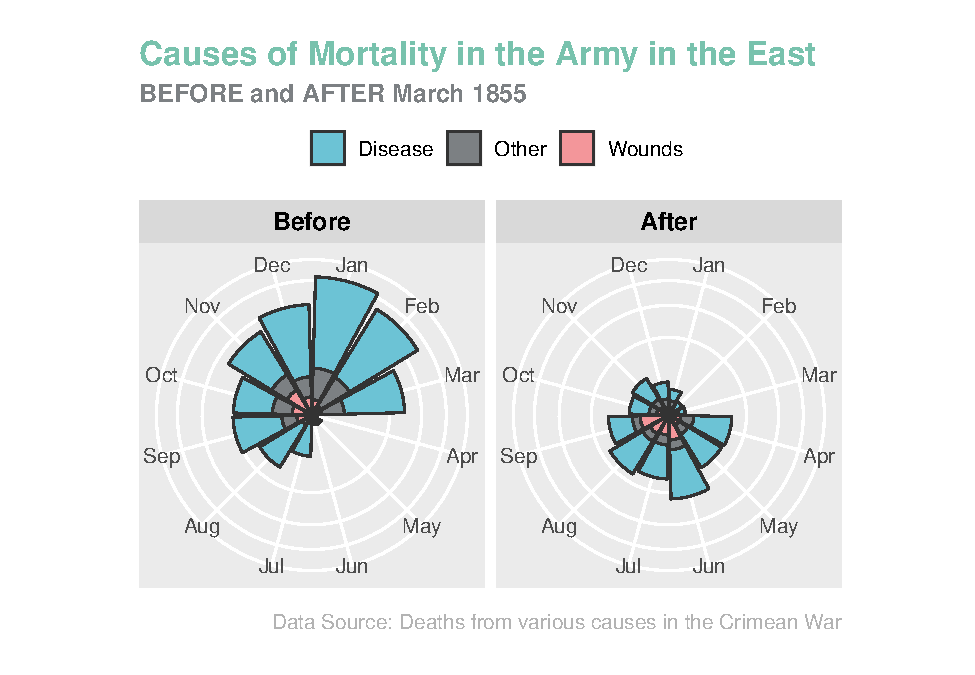
\includegraphics[width=0.9\linewidth]{Byler_Nightingale-Final-Project_Writeup_files/figure-latex/modern rose1-1} \end{flushleft}

\newpage

\hypertarget{combined-rose-diagram-24-months}{%
\subsubsection{\texorpdfstring{\emph{Combined Rose Diagram: 24
Months}}{Combined Rose Diagram: 24 Months}}\label{combined-rose-diagram-24-months}}

Next, I wanted to try to create a single rose diagram that shows all two
years of data on a single set of coordinates, as though it were a
24-hour clock. Additionally, it would only show the changes in the death
rate from disease, since Nightingale was most interested in preventable
deaths. I was inspired by this
\href{https://www.r-bloggers.com/2013/01/going-beyond-florence-nightingales-data-diagram-did-flo-blow-it-with-wedges/}{site}.
However, I could not get their code to work, so I modified my rose
diagram code from above instead.

\begin{Shaded}
\begin{Highlighting}[]
\CommentTok{\# CREATE SUBSET FOR COMBINED ROSE DIAGRAM}
\NormalTok{long\_data }\SpecialCharTok{\%\textgreater{}\%}
    \FunctionTok{select}\NormalTok{(}\SpecialCharTok{{-}}\FunctionTok{c}\NormalTok{(}\StringTok{"Date"}\NormalTok{, }\StringTok{"Month\_Year"}\NormalTok{, }\StringTok{"Month"}\NormalTok{, }\StringTok{"Year"}\NormalTok{,}
        \StringTok{"Army"}\NormalTok{, }\StringTok{"Rate"}\NormalTok{, }\StringTok{"mo"}\NormalTok{)) }\SpecialCharTok{\%\textgreater{}\%}
    \FunctionTok{subset}\NormalTok{(Cause }\SpecialCharTok{==} \StringTok{"Disease"}\NormalTok{) }\OtherTok{{-}\textgreater{}}\NormalTok{ sub\_long}
\end{Highlighting}
\end{Shaded}

\begin{Shaded}
\begin{Highlighting}[]
\CommentTok{\# COMBINED ROSE DIAGRAM}
\NormalTok{sub\_long }\SpecialCharTok{\%\textgreater{}\%}
    \FunctionTok{ggplot}\NormalTok{(}\FunctionTok{aes}\NormalTok{(}\AttributeTok{x =} \FunctionTok{factor}\NormalTok{(Sort\_Date), }\AttributeTok{y =}\NormalTok{ Deaths, }\AttributeTok{fill =}\NormalTok{ Regime)) }\SpecialCharTok{+}
    \FunctionTok{geom\_col}\NormalTok{(}\AttributeTok{color =} \StringTok{"grey20"}\NormalTok{) }\SpecialCharTok{+} \FunctionTok{scale\_fill\_manual}\NormalTok{(}\AttributeTok{values =} \FunctionTok{c}\NormalTok{(}\StringTok{"\#6cc3d5"}\NormalTok{,}
    \StringTok{"\#4b8c99"}\NormalTok{), }\AttributeTok{name =} \StringTok{""}\NormalTok{) }\SpecialCharTok{+} \FunctionTok{scale\_y\_sqrt}\NormalTok{() }\SpecialCharTok{+} \FunctionTok{coord\_equal}\NormalTok{(}\AttributeTok{ratio =} \DecValTok{1}\NormalTok{) }\SpecialCharTok{+}
    \FunctionTok{coord\_polar}\NormalTok{() }\SpecialCharTok{+} \FunctionTok{labs}\NormalTok{(}\AttributeTok{title =} \StringTok{"Deaths from Preventable Causes"}\NormalTok{,}
    \AttributeTok{subtitle =} \StringTok{"BEFORE and AFTER March 1855"}\NormalTok{) }\SpecialCharTok{+} \FunctionTok{theme}\NormalTok{(}\AttributeTok{legend.position =} \StringTok{"top"}\NormalTok{) }\SpecialCharTok{+}
    \FunctionTok{theme}\NormalTok{(}\AttributeTok{text =} \FunctionTok{element\_text}\NormalTok{(}\AttributeTok{size =} \DecValTok{10}\NormalTok{)) }\SpecialCharTok{+} \FunctionTok{theme}\NormalTok{(}\AttributeTok{axis.title.x =} \FunctionTok{element\_blank}\NormalTok{()) }\SpecialCharTok{+}
    \FunctionTok{theme}\NormalTok{(}\AttributeTok{axis.title.y =} \FunctionTok{element\_blank}\NormalTok{()) }\SpecialCharTok{+} \FunctionTok{theme}\NormalTok{(}\AttributeTok{axis.text.y =} \FunctionTok{element\_blank}\NormalTok{()) }\SpecialCharTok{+}
    \FunctionTok{theme}\NormalTok{(}\AttributeTok{axis.ticks =} \FunctionTok{element\_blank}\NormalTok{()) }\SpecialCharTok{+} \FunctionTok{theme}\NormalTok{(}\AttributeTok{plot.margin =} \FunctionTok{unit}\NormalTok{(}\FunctionTok{rep}\NormalTok{(}\FloatTok{0.7}\NormalTok{,}
    \DecValTok{4}\NormalTok{), }\StringTok{"cm"}\NormalTok{)) }\SpecialCharTok{+} \FunctionTok{theme}\NormalTok{(}\AttributeTok{plot.title =} \FunctionTok{element\_text}\NormalTok{(}\AttributeTok{color =} \StringTok{"\#78c2ad"}\NormalTok{,}
    \AttributeTok{size =} \DecValTok{16}\NormalTok{, }\AttributeTok{face =} \StringTok{"bold"}\NormalTok{)) }\SpecialCharTok{+} \FunctionTok{theme}\NormalTok{(}\AttributeTok{plot.subtitle =} \FunctionTok{element\_text}\NormalTok{(}\AttributeTok{color =} \StringTok{"\#7C8083"}\NormalTok{,}
    \AttributeTok{size =} \DecValTok{12}\NormalTok{, }\AttributeTok{face =} \StringTok{"bold"}\NormalTok{)) }\SpecialCharTok{+} \FunctionTok{theme}\NormalTok{(}\AttributeTok{legend.text =} \FunctionTok{element\_text}\NormalTok{(}\AttributeTok{color =} \StringTok{"black"}\NormalTok{,}
    \AttributeTok{size =} \DecValTok{10}\NormalTok{))}
\end{Highlighting}
\end{Shaded}

\begin{flushleft}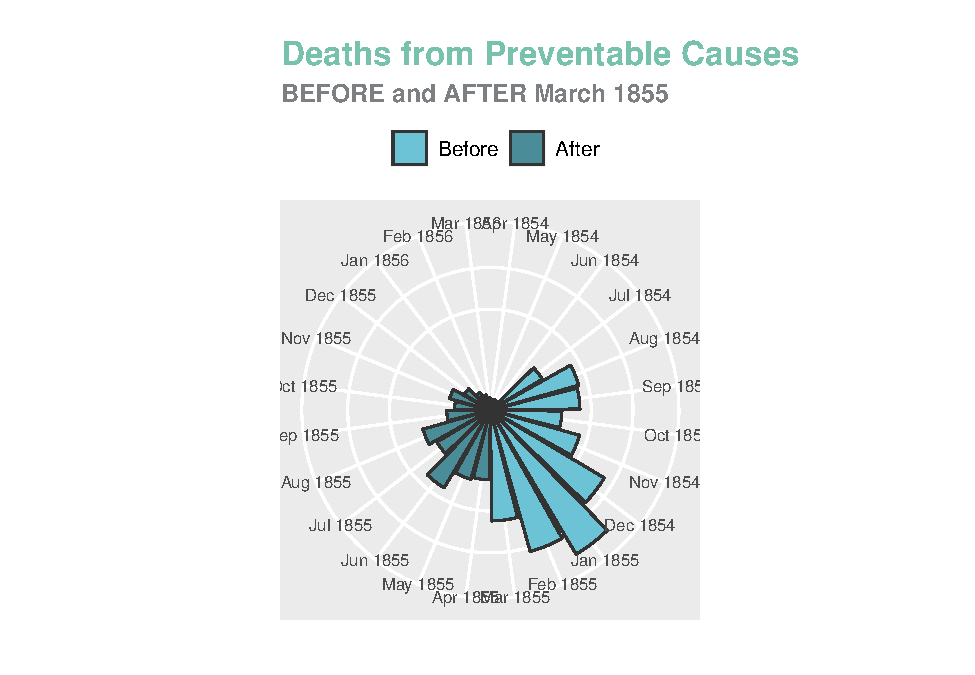
\includegraphics[width=0.9\linewidth]{Byler_Nightingale-Final-Project_Writeup_files/figure-latex/combo rose-1} \end{flushleft}

I also created two modern charts using the same dataset: a bar chart
comparing deaths from all three causes (\texttt{Disease},
\texttt{Wounds}, \texttt{Other}) between the ``\emph{Before}'' period
and the ``\emph{After}'' period, and a line chart that explores the
trend in preventable deaths from disease over the two year period. These
charts can be seen on the Shiny app website:
\url{https://e11i3n0r.shinyapps.io/631-EllieByler-FinalProject/}

\hypertarget{section-8}{%
\section{\texorpdfstring{\textcolor{WildStrawberry}{TOPICS FROM CLASS}}{}}\label{section-8}}

\hypertarget{section-9}{%
\subsection{\texorpdfstring{\textcolor{TealBlue}{1. Github:}}{}}\label{section-9}}

Github is a skill that I had been meaning to learn at some point, but I
never had a good opportunity to do it until this class. There are still
many mysteries to be uncovered, but I have gotten the hang of using
\texttt{push} and \texttt{pull} for version control management. Having a
Github account set up will be useful for any future coding projects I
do, and I like having the project for this course publicly available in
case I would like to use it in a portfolio.

\hypertarget{section-10}{%
\subsection{\texorpdfstring{\textcolor{TealBlue}{2. R Markdown:}}{}}\label{section-10}}

We have obviously been using R Markdown all semester, and I've really
gotten the hang of it. However, I never realized how specific of a
coding style it is until I had been working on my Shiny app code for a
while and then switched back to R Markdown. Markdown has some very
specific syntax, and I had to modify some of my app code to get it to
work in the pdf. I've used flavors of Markdown on other sites (e.g.,
Discord and Slack use some variation of Markdown to let you format text
as bold, italic, etc.).

\hypertarget{section-11}{%
\subsection{\texorpdfstring{\textcolor{TealBlue}{3. R Shiny:}}{}}\label{section-11}}

This project wouldn't have existed without R Shiny. We didn't cover this
topic in class, but I had noticed the option in the File menu to create
a Shiny Web App, and I was excited to learn more. As the minimal
functional code above shows, the basics of Shiny app creation are super
simple to master. It took a little more trial-and-error and tutorials to
figure out exactly what to include where to make the app look how I
wanted, but there were numerous detailed web resources. I thought it was
interesting that a lot of the code is actually html that is generated by
R.

\hypertarget{section-12}{%
\subsection{\texorpdfstring{\textcolor{TealBlue}{4. Tidyverse (ggplot2, dplyr, tidyr, stringr, etc.):}}{}}\label{section-12}}

The tidyverse package was integral to my project. The time we spent in
class going over how to use \texttt{ggplot} aided my comprehension of
the code for the rose diagram and how I would need to modify it to make
a combined rose diagram. It also made it easy to add a grouped bar chart
and a paneled line chart (using \texttt{facet\_wrap}). The original
dataset was clean, but it was far from normalized or ``tidy'' and this
package made it almost as easy to pivot the data in R as it would be in
Excel.

There are other packages I used that are associated with the tidyverse
but need to be installed separately. These include \texttt{readxl} for
loading in the \texttt{.xlsx} data, \texttt{lubridate} for handling
dates, and \texttt{magrittr} for providing the special tidyverse pipe
\texttt{\%\textgreater{}\%}.

\hypertarget{section-13}{%
\subsection{\texorpdfstring{\textcolor{TealBlue}{5. Assorted other topics: Regex, MathJax, Bootstrap, etc.:}}{}}\label{section-13}}

I was a little surprised by how many other topics I ended up using in my
project. These were topics that weren't covered in class, but are easy
enough to figure out once you have experience with R. I used
\texttt{regex} in my data preparation to assign the variable
\texttt{Regime} to the records based on their date.

\begin{Shaded}
\begin{Highlighting}[]
\FunctionTok{mutate}\NormalTok{(}\AttributeTok{Regime =} \FunctionTok{if\_else}\NormalTok{(}\FunctionTok{str\_detect}\NormalTok{(.}\SpecialCharTok{$}\NormalTok{Month\_Year, }\StringTok{"[:alpha:]}\SpecialCharTok{\textbackslash{}\textbackslash{}}\StringTok{s1854"}\NormalTok{),}
    \StringTok{"Before"}\NormalTok{, }\FunctionTok{if\_else}\NormalTok{(}\FunctionTok{str\_detect}\NormalTok{(.}\SpecialCharTok{$}\NormalTok{Month\_Year, }\StringTok{"(Jan|Feb|Mar)}\SpecialCharTok{\textbackslash{}\textbackslash{}}\StringTok{s1855"}\NormalTok{),}
        \StringTok{"Before"}\NormalTok{, }\StringTok{"After"}\NormalTok{)))}
\end{Highlighting}
\end{Shaded}

I used \texttt{MathJax} to format an inline equation like one would with
\texttt{LaTeX}.

\begin{center}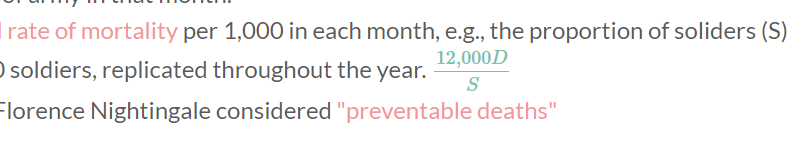
\includegraphics[width=0.9\linewidth]{mathjax_display} \end{center}

\begin{center}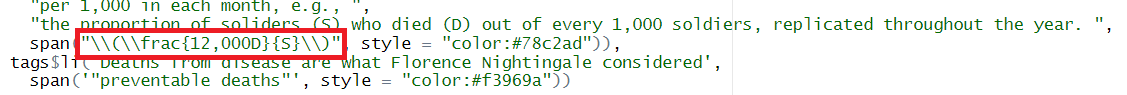
\includegraphics[width=0.9\linewidth]{mathjax_code} \end{center}

And lastly, I used Bootstrap to customize my website using the object
\texttt{bslib::bs\_theme()} and a theme called ``Minty'' from
\href{https://bootswatch.com/}{bootswatch.com}.

\hypertarget{section-14}{%
\section{\texorpdfstring{\textcolor{WildStrawberry}{CONCLUSION}}{}}\label{section-14}}

Overall, I am very pleased with how this app turned out. I've created
websites before using website creation platforms before, but this is the
first time I've made a page that I coded from scratch. There are some
issues with the layout that I would fix if I had more time, for instance
the picture slideshow on the Introduction page looks bad if the screen
is too narrow, which would be a problem for mobile phones. Shiny has
options to make a layout more responsive, but then you have to sacrifice
having the charts look exactly how you want. I also would have loved to
make the app more interactive based on user input using Shiny's
\href{https://shiny.rstudio.com/gallery/widget-gallery.html}{widget
gallery}, however I discovered that with the dataset I chose, the user
wouldn't gain much additional insight by being able to (i.e.) select the
year from a drop-down menu. Other datasets would be better suited to
selection inputs. As a trade-off, I instead focused on making the site
as user-friendly as possible, with aesthetic design, informational
videos, clearly labeled navigation panel, and tables that let the user
examine the datasets for themselves. In the end, the important thing is
that I accomplished my goal of creating a functioning R Shiny app that
recreates Florence Nightingale's rose diagram, explains the historical
context, and leaves the user with a better appreciation of this
remarkable woman.

\newpage

\hypertarget{section-15}{%
\section{\texorpdfstring{\textcolor{WildStrawberry}{SOURCES}}{}}\label{section-15}}

\begin{itemize}
\tightlist
\item
  \textbf{Mathematics of the Coxcombs:}\\
  \url{http://understandinguncertainty.org/node/214}

  \begin{itemize}
  \tightlist
  \item
    Explains how rose/coxcomb/polar area charts work, as well as how
    Florence calculated death rate as ``annual rate of mortality per
    1000 in each month''
  \end{itemize}
\item
  \textbf{Florence Nightingale's Rose Diagram:}\\
  \url{https://rpubs.com/chidungkt/819554}

  \begin{itemize}
  \tightlist
  \item
    Inspiration and code base for modern recreation of rose diagram.
  \end{itemize}
\item
  \textbf{Nightingale Dataset:}\\
  \url{https://github.com/vincentarelbundock/Rdatasets/blob/master/csv/HistData/Nightingale.csv}

  \begin{itemize}
  \tightlist
  \item
    Original dataset from Github.
  \end{itemize}
\item
  \textbf{Wikipedia: Florence Nightingale:}\\
  \url{https://en.wikipedia.org/wiki/Florence_Nightingale}

  \begin{itemize}
  \tightlist
  \item
    Source of Florence Nightingale portraits and sound recording.
  \end{itemize}
\item
  \textbf{Bootswatch Themes: Minty:}\\
  \url{https://bootswatch.com/minty/}

  \begin{itemize}
  \tightlist
  \item
    Theme for Shiny app.
  \end{itemize}
\item
  \textbf{Going Beyond Florence Nightingale's Data Diagram: Did Flo Blow
  It with Wedges?:}\\
  \url{https://www.r-bloggers.com/2013/01/going-beyond-florence-nightingales-data-diagram-did-flo-blow-it-with-wedges/}

  \begin{itemize}
  \tightlist
  \item
    Inspiration and code base for combined rose diagram.
  \end{itemize}
\item
  \textbf{Florence Nightingale's Forgotten Legacy: Public Health
  laws:}\\
  \url{http://www.florence-nightingale-avenging-angel.co.uk/blog/?page_id=462}

  \begin{itemize}
  \tightlist
  \item
    Historian explains the rose diagram.
  \end{itemize}
\end{itemize}

\end{document}
